\section{Introduction}
\subsection{Présentation du projet}
Le COPEVUE a lancé un appel d'offre dans le cadre de la réalisation d'un système de monitoring de sites isolés. Il s'agit donc de concevoir en premier lieu une solution technique permettant de répondre au mieux aux exigences fonctionnelles et non fonctionnelles que le COPEVUE formule. De façon synthétique notre équipe va proposer une solution permettant de surveiller des sites naturels difficiles d'accès (souvent à cause des conditions environnementales) et peu peuplés. Dans ces sites isolés sont souvent regroupés des postes de travail et ces zones doivent pouvoir être surveillées en dépit de la distance qui les sépare du bureau de contrôle.

\subsection{Présentation du document}
Ce document présente le cahier des charges du logiciel permettant la supervision centralisée de tous les site isolés surveillés,c'est à dire la définition des spécifités du logiciel qui sera développé. C'est une formalisation des besoins exprimés par la MOA et permet de s'assurer que les différents parties se comprennent sur le``quoi''. Ce document servira de référence à la MOE et la MOA pour les phases suivantes du projet.

\subsection{Documents applicables / Documents de référence}
\begin{itemize}
	\item Cours de Génie Logiciel
	\item Cours de Qualité Logiciel
	\item Manuel Qualité 
	\item Etude de faisabilité
	\item Spécification technique des besoins
\end{itemize}

\subsection{Terminologie et abréviations}
\begin{itemize}
	\item CdC : cahier des charges.
	\item MOA : maîtrise d'ouvrage.
	\item MOE : maîtrise d'ouvrage.
	\item MVC : pattern de conception Modèle-Vue-Contrôleur qui permet un découpage entre les différents modules d'une application.
	\item Système central : Serveur principal de la solution technique. Récupère les données depuis l'ensemble des sites isolés, et permet leur consultation ainsi que de la prise de décisions depuis un portail en ligne.
	\item Station du site isolé : Point central d'un site, est composée d'un système embarqué, de batteries, et de moyens de communications avec les capteurs, et avec le système central.
\end{itemize}

\section{Présentation du problème}
\subsection{Buts, nature du logiciel, utilisateurs concernés}
L'objectif est de fournir une interface qui permette de suivre les informations dont on dispose sur les différents sites actuellement surveillés par notre système comme le niveau de liquide dans une cuve ou le niveau de remplissage des containers, de manière efficace et simple. Il offrira également la possibilité de reconfigurer certains paramètres du système pour faire de la maintenance à distance (modification du niveau d'alerte, cycle de d'envoi des données, ...)
Lorsque la situation est critique sur un site, l'utilisateur doit en être avertis par un affichage approprié pour prendre les décisions qui s'imposent.

\subsection{Formulation des besoins, exploitation et ergonomie, expérience}

\subsubsection{Authentification}
La connexion au serveur centrale doit se faire de manière sécurisé et authentifié, afin de sécuriser l'ensemble.

\subsubsection{Récupération des données}
Après que l'utilisateur se soit authentifié, toutes les données seront téléchargées depuis le serveur central pour être stocké en local, afin d'éviter d'avoir à les télécharger de nouveau en cas de perte de connexion. Les données téléchargés sont :
\begin{itemize}
\item La valeur des mesures effectuées depuis la dernière transmission par chacun des capteurs. La quantité de valeurs dépend de la granularité avec laquelle est configurée le site. Chaque valeur sera bien évidemment horodatée.
\item L'état physique et logique de la station et du site. Cela peut comprendre la température ambiante, l'autonomie estimée des différentes batteries, les logs systèmes engrangés par le système informatique, etc.
\item L'identification du site et des différents capteurs. % A voir.
\end{itemize}
La récupération se fera grâce à l'API qu'exposera le serveur centrale, décrite plus en détail dans le dossier ``APIs et Interfaces''. Tous les transferts sont bien sûr sécurisés.

\subsubsection{Visualisation}
Il s'agit du besoin principal de ce sous-système, qui doit permettre à l'utilisateur de superviser l'ensemble des sites isolés de manière efficace et sûr. Pour faciliter sa tâche, différents niveau de visualisation seront offerts:
\begin{itemize}
	\item L'affichage général de l'ensemble des sites présents le monde avec leur localisation, avec une mise en évidence des sites dans un état critique, pour aider l'utilisateur dans sa prise de décision.
	\item L'affichage des données physiques ( niveau de liquide, état des batteries,...) d'un capteur que l'utilisateur aura sélectionné parmi tous les capteurs d'un site.
	\item L'affichage de l'historique des données d'un capteur pour gagner en traçabilité sur l'évolution d'un site.
	\item L'affichage la liste des capteurs d'un site pour la sélection des capteurs mais aussi pour donner de manière condensé les informations sur un site.
	\item L'affichage des paramètres de configuration actuelle de la station d'un site afin de pouvoir vérifier et attester son bon paramétrage.
	\item L'affichage de l'historique de paramétrage pour la traçabilité de l'évolution éventuelle des configurations.
\end{itemize}

\subsubsection{Configuration}
Dans l'objectif d'optimiser le processus de maintenance, si elle peut être effectuée à distance, le logiciel de supervision offrira également des possibilités de configuration.
L'utilisateur disposera d'interfaces pour modifier:
\begin{itemize}
	\item Les différents quantum de temps définissant la granularité avec laquelle la station du site isolé effectue ses mesures et en transmet les résultats au système central.
	\item Les fréquences de transmission satellite utilisées par le présent sous-système.
	\item Des paramètres systèmes tels que le niveau de logs à engranger et à transmettre, les politiques de reprise sur échec (dans le contexte de la communication avec les capteurs par exemple).
	\item Des données de configuration spécifiques à certains capteurs, qui leur seront transmis à leur prochaine connexion (les intervalles de relevés comme mentionné plus haut, mais aussi des paramètres spécifiques à un type de capteur tels que les fréquences d'ultrasons à utiliser pour effectuer un relevé de remplissage d'une cuve).
\end{itemize}

\subsubsection{Expérience utlisateur}
On attachera également une grande importance à la facilité d'apprentissage et d'utilisation, car l'utilisateur finale n'a pas forcément une grande connaissance dans le maniement des outils informatiques. Il n'est pas souhaitable qu'une formation soit nécessaire pour l'utilisation de ce nouvel outil.

\subsection{Portée, développement, mise en oeuvre, organisation de la maintenance}
Le développement du logiciel se fera en Java avec un modèle MVC, en utilisant les méthodes agiles, afin d'avoir un retour-utlisateur le plus tôt possible, pour minimiser le risque d'avoir un logiciel qui ne sera pas accepté et diminuer ainsi les besoins de maintenance. Ce type de développement offre également l'avantage de rassurer la MOA qui peut voir une réalisation concrète très rapidement avec la possibilité de réagir très rapidement pour la MOE si ce qui est fait ne correspond pas aux attentes et cette méthode semble particulièrement adapté vu la taille relativement faible en terme de développement de ce sous-système. 
Pour faciliter la future maintenance, on veillera à fournir une documentation suffissante tant sur l'application à proprement parlé que sur les tests effectués.

\subsection{Limites}
Si aucune connexion avec le serveur central ne peut être établie, le logiciel n'est pas fonctionnel, dans le sens où seul la configuration au serveur central est possible.

\section{Exigences fonctionnelles}
\subsection{Fonctions de base, performances et aptitudes}
On distinguera les fonctions principales suivantes:
\begin{itemize}
	\item authentification pour accéder aux serveurs,
	\item affichage d'une carte avec la localisation des différents sites sur une carte,
	\item affichage de l'état d'un capteurs
	\item affichage de l'état de la base,
	\item affichage de la valeur d'un capteur,
	\item configuration de la base,
	\item configuration d'un capteur,
	\item affichage de l'historique des données,
	\item affichage de l'historique de paramétrages,
\end{itemize}

Au niveau des performances, on offrira une application fluide, sans aucun processus bloquant pour l'interface, pour ne pas gêner l'utilisateur et surtout lui offrir une expérience de navigation rapide et fluide.

\subsection{Contraintes d'utilisation}
La seule contrainte est d'avoir un accès au serveur central par Internet.

\subsection{Critères d'appréciation de la réalisation effective de la fonction}

\begin{tabular}{|c|c|c|}
	\hline Fonction & Nécessité & Difficulté d'implémentation\\
	\hline 
	 Authentification & 9 & 5\\
	 Affichage des sites sur une carte & 9 & 5\\
	 Affichage de l'état d'un capteur & 9 & 5\\
	 Affichage de l'état de la base & 9 & 5\\
	 Affichage de la valeur d'un capteur & 9 & 5\\
	 Configuration de la base & 9 & 5\\
	 Configuration d'un capteur & 9 & 5\\
	 Affichage de l'historique des données & 9 & 5\\
	 Affichage de l'historique de paramétrage & 9 & 5\\
	\hline
\end{tabular}

%\subsection{Flexibilité dans la façon de mettre en oeuvre la fonction convercée, variation de coûts associée en fonction de cette flexibilité}

\section{Exigences non fonctionnelles}
\subsection{Sécurité}
Il faut que l'accès aux paramétrages des stations soient sécurisés pour éviter toute mauvaise configuration qui pourrait nuire à la pérennité du sytème.

\subsection{Fiabilité}
La fiabilité de l'application installé doit être bonne, avec une résistance aux erreurs, pour éviter de paralyser la prise de décision.

\subsection{Portabilité}
Pour que le logiciel soit installable sur différents configurations matérielles ou logicielles (systèmes d'exploitation différents), le logiciel sera développé dans un langage de haut niveau qui sera executé sur la machine virtuelle de l'ordinateur cible. On a choisit Java car c'est un langage très largement utilisé.

\subsection{Ergonoomie}
Le logiciel doit être le plus ergonomique possible pour faciliter la prise en main et avoir un haut niveau d'acceptation auprès des utilisateurs finaux. L'objectif est de fournir un logiciel dont la prise en main ne nécessitera aucune formation, mais juste le temps de parcourir les différentes fenêtres.

\subsection{Modularité}
En séparant distinctement les différents couches d'acquisition de données (auprès d'un autre module) de l'affichage, pour permettre une maintenance plus facile et évolutive en cas d'évolution future.

\section{Contraintes imposées, faisabilité technologique, moyens}
\subsection{Sûreté, planning, organisation, communication}

\subsection{Complexité}
Pour ce sous-système, il n'y a pas vraiment de complexité, aucun traitement n'étant fait et il existe des outils pour le développement d'interface.

\subsection{Compétences, moyens et règles}
Les compétences nécessaires à la réalisation du projet :

\begin{itemize}
\item Connaissances en ergonomie.
\item Programmation Java.
\item Connaissance du patron de conception MVC.
\end{itemize}

\subsection{Normes de documentation}
Les normes de documentation à adopter sont décrites dans le plan d'assurance qualité commun aux différents éléments de ce projets.

\section{Configuration cible}
\subsection{Matériels et logiciels}
La configuration minimale pour le bon fonctionnement du logiciel : 
\begin{itemize}
	\item un PC avec un processeur de 233 MHz minimum ou de capacité supérieure (recommandé), de la famille Intel Pentium/Celeron ou famille AMD K6/Athlon/Duron,
	\item 128 Mo de RAM ou plus recommandé,
	\item 150 Mo d'espace disque disponible ;
	\item une carte vidéo (graphique) et un moniteur Super VGA (800x600) ou de résolution supérieure,
	\item un clavier et une souris,
	\item Windows XP sp1 ou Ubuntu 6.0 ou Mac OS 10.0 installé,
	\item Java 1.5 installé.
\end{itemize}

\subsection{Stabilité de la configuration}
Lors de futur évolution, on veillera à ce que la configuration minimale n'évolue pas ou peu, sachant que la configuration minimale requise équivaut au matériel informatique disponible dans les années 2000.

\subsection{Description des API}
Ce sous-système n'expose aucune API, il y fait seulement appel.

\section{Guide de réponse au cahier des charges}


\section{Annexes}
\subsection{Observations de l'existant}
\subsection{Propositions d'orientation}

\subsection{Images d'écrans principaux du logiciel}

\begin{figure}[hb]
  \centering
  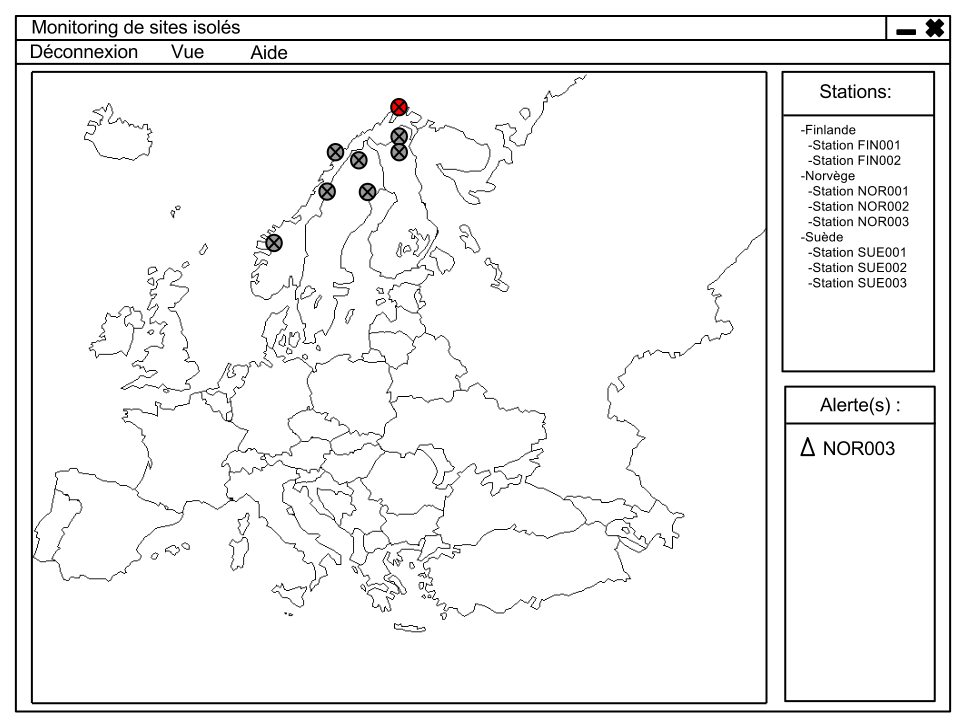
\includegraphics[width=15cm]{Supervision/InterfaceSupervision1.png}
  \caption[Ebauche de l'interface pour la fenêtre de supervision global.]%
  {Ebauche de l'interface pour la fenêtre de supervision global.}
\end{figure}

\begin{figure}[hb]
  \centering
  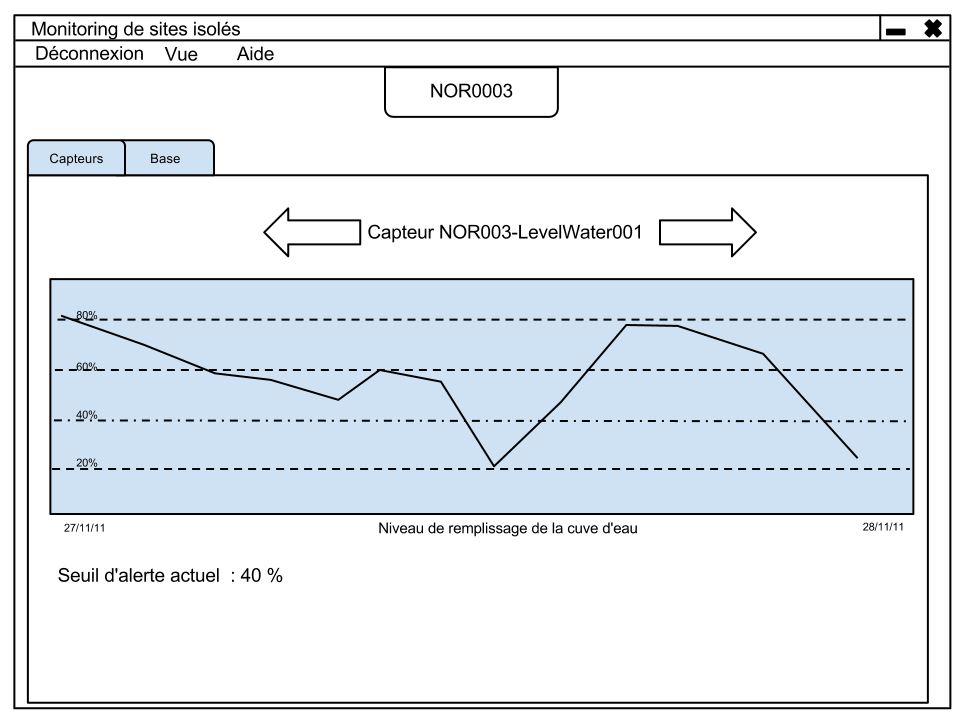
\includegraphics[width=15cm]{Supervision/InterfaceSupervision2.png}
  \caption[Ebauche de l'interface pour la fenêtre de visualisation de l'évolution des valeurs d'un capteur.]%
  {Ebauche de l'interface pour la fenêtre de visualisation de l'évolution des valeurs d'un capteur.}
\end{figure}
 
\subsection{Résultat de l'analyse de la valeur}